En Carles vol construir un decorat per a l'obra de teatre de final de curs en forma d'un rectangle i dos
semicercles, tal com es mostra a la figura següent:
\begin{center}
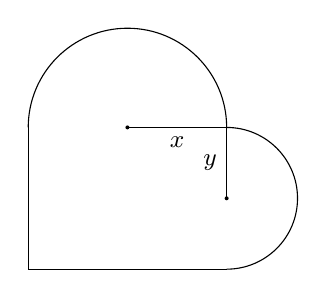
\begin{tikzpicture}[scale=0.9]
  \draw (0,0) -- (2.8,0);
  \draw (0,0) -- (0,2);
  \draw (0,2) arc[start angle=180,end angle=0,radius=1.4];
  \draw (2.8,0) arc[start angle=-90,end angle=90,radius=1];
  \draw[thin] (1.4,2) -- (2.8,2);
  \draw[thin] (2.8,1) -- (2.8,2);
  \fill (1.4,2) circle (0.8pt);
  \fill (2.8,1) circle (0.8pt);
  \node[below,font=\small] at (2.1,2) {$x$};
  \node[left,font=\small] at (2.8,1.5) {$y$};
\end{tikzpicture}
\end{center}

\begin{apartats}

\apartat{1}
Determineu el perímetre i l'àrea del decorat que s'ha de construir en funció de $x$ i de $y$.

\begin{solucio}
Tal com s'indica a la figura, el radi de la semicircumferència superior és $x$, i el de la lateral, $y$. Per tant,
el perímetre de la figura serà
\[
P(x,y)=2x+2y+\frac{2\pi x}{2}+\frac{2\pi y}{2}=(2+\pi)(x+y),
\]
i la seva àrea,
\[
A(x,y)=\frac{\pi x^2}{2}+\frac{\pi y^2}{2}+4xy .
\]

\textit{Pauta oficial:} 0,5 per l'expressió del perímetre, i 0,5 per la de l'àrea (no importa si el resultat el
donen més o menys simplificat).
\end{solucio}

\apartat{1,5}
Per a revestir el perímetre del decorat, en Carles té material per a cobrir fins a 10 m. Si el vol gastar tot,
quines seran les mides del decorat d'àrea màxima que podrà construir? Quin és el valor d'aquesta àrea?

\begin{solucio}
Com que volem $P(x,y)=(2+\pi)(x+y)=10$, tenim $y=\frac{10}{2+\pi}-x$. Substituint-ho a l'expressió de l'àrea,
obtenim
\[
A(x)=\frac{\pi x^2}{2}+\frac\pi2\left(\frac{10}{2+\pi}-x\right)^2+4x\left(\frac{10}{2+\pi}-x\right)
=\frac{\pi x^2}{2}+\frac\pi2\left(\frac{10}{2+\pi}-x\right)^2+\frac{40x}{2+\pi}-4x^2 .
\]
Derivant i igualant a zero, obtenim
\[
A'(x)=\pi x-\pi\left(\frac{10}{2+\pi}-x\right)+\frac{40}{2+\pi}-8x=0,
\]
\[
(2\pi-8)x=\frac{10\pi-40}{\pi+2}\;\rightarrow\;x=\frac{10\pi-40}{(\pi+2)(2\pi-8)}=0{,}972\ldots\ \text{m}.
\]
Ara comprovem que és un màxim, veient que $A''=2\pi-8<0$. Per tant, el decorat d'àrea màxima possible és un
quadrat de dimensions $x=0{,}972\ldots$ m i $y=\frac{10}{2+\pi}-x=0{,}972\ldots$ m. Finalment, el valor d'aquesta
àrea màxima és $A(0{,}972)=6{,}747\ldots\ \text{m}^2$.

\textit{Pauta oficial:} 0,5 per l'expressió de la funció a derivar, 0,25 per la derivada, 0,25 per la solució,
0,25 per comprovar que és un màxim, i 0,25 per la resposta final.

\textit{Nota del banc:} simplificant, $x=y=\frac{5}{\pi+2}\approx0{,}9725$ m (el rectangle és un quadrat de
$2x\approx1{,}945$ m de costat), i l'àrea màxima exacta és
$\frac{25(\pi+4)}{(\pi+2)^2}\approx6{,}754\ \text{m}^2$. El $6{,}747\ldots$ del criteri surt de prendre $x$ i
$y$ tots dos arrodonits a 0,972. Totes dues respostes són correctes.
\end{solucio}

\end{apartats}
